  \documentclass[11pt]{article}

  \usepackage{fullpage}
  \usepackage{graphicx}
  \graphicspath{ {./images/} }
  \begin{document}

  \title{ARM Checkpoint Report}
  \author{Otto White, Paulo Lemos, Robert Stok, Weizhong Zhao}

  \maketitle

  \section*{Group Organisation}

  \subsection*{How we split the work}

After reviewing the specification together, we decided to split the emulator task into three  sections: creating general file and program structure, loader and fetch-decode-execute functions, and the four ARM instructions. We worked on setting programming standards and general program/file structure as a group as this would form the basis of our entire emulator. Next, we allocated the loader and fetch functions to one pair (Weizhong and Paulo) and the decode and execute functions to another (Otto and Rob). The final four instructions were distributed to each member as follows: data processing to Otto, multiply to Rob, single data transfer to Paulo and branch to Weizhong. Once all were completed, we came together to merge our seperate branches. Debugging and final testing was then performed by Otto.

  \subsection*{How well the group is working}

For the majority of the emulator work, communication was carried out through online meetings and messaging due to schedule and location differences. Despite this, we were still able to work efficiently as we had set up internal deadlines and allocated tasks early on. By working on general program structure and writing reusable code such as definitions.h together, each of us benefited from having a strong understanding of the emulator as a whole and how different parts fit together. We distributed tasks by function but we quickly realised that some parts were more complicated than others which resulted in varying amounts of workload. For the assembler, we plan to be more flexible and let those who finish their tasks earlier help with others. While pair programming was useful in ensuring code correctness, we found it slower than solo programming which we plan to do for most of the assembler. To compensate for no longer pair programming, we will create a comprehensive testing system for our assembler (more details below). Overall, we feel our group has been working well and completing objectives in a timely manner.

  \section*{Implementation Strategies}

  \subsection*{Emulator Structure}

Our emulator is structured as below. At the top level we have the emulate.c file which runs the main process. Here, we create an emulated system of memory and registers in the form of a struct which is stored on the heap and populated with zeroes. The instructions are loaded into our emulated memory using the loader function implemented in loader.c. We then call the pipeline function defined in pipeline.c, and pass our emulated state struct. The pipeline function runs the execute, decode and fetch stages in this order as it reduces unnecessary computation when a branch instruction is executed: it allows us to skip the fetch and decode stages since branch flushes the pipeline anyway. This order also creates a pipeline-like execution flow with minimal usage of memory, since the data in each stage can be directly passed to the next one without needing to be saved in temporary variables. In the fetch phase, a pointer to the struct state is passed into the fetch function implemented in fetch.c: this obtains the next instruction stored at the memory location held in the PC and returns it as a 32 bit binary number. In the decode phase, a pointer to the state struct and our 32 bit binary instruction are passed to the decode function in decode.c, and a descriptive instruction struct is returned. In the execute phase, a pointer to the state and a pointer to the Instruction struct are passed into the execute function defined in execute.c. To avoid code duplication across the instruction functions, condition checking to determine whether each instruction should be run is done in execute. Execute then checks the type of instruction held in the instruction struct and passes both a pointer to the instruction struct and a pointer to the state struct to one of the four instructions. These are handled by the functions implemented in data/_processing.c, multiply.c, single/_data/_transfer.c or the branch.c, which will side effect the state struct accordingly. The functions inside these files are all defined in the instructions.h file, which is included by pipeline.c. All the files also rely on the definitions.h file to define the State struct, Instruction struct as well as the Instruction/_type, Opcode, and Condition enums, which are used in the Instruction struct. 

 \begin{figure}[h]
 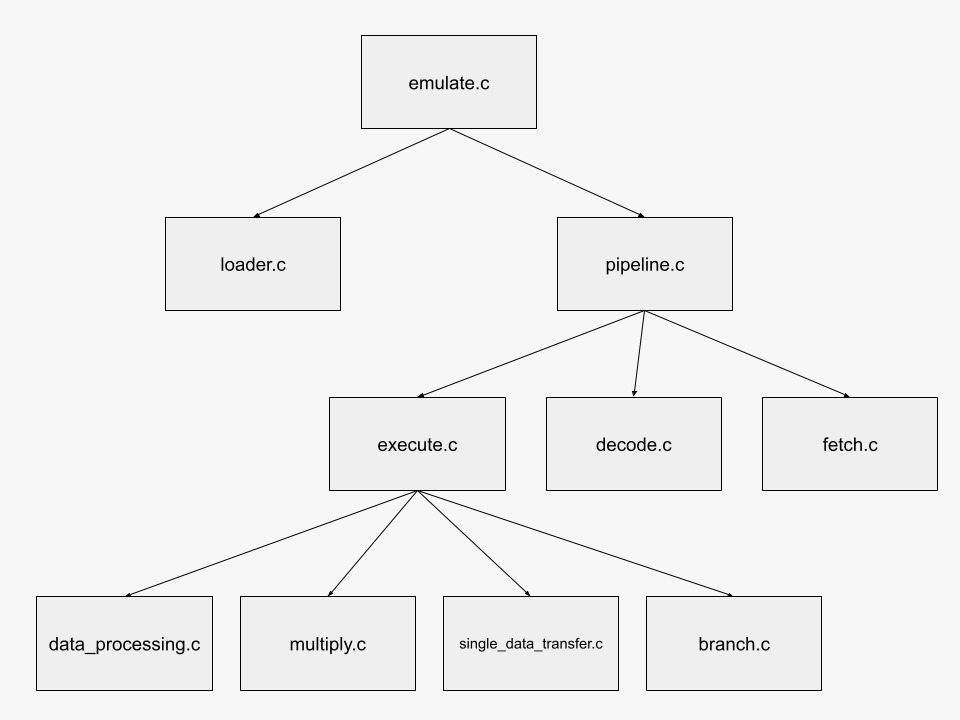
\includegraphics[scale=0.4]{emulator_structure}
 \centering
 \end{figure}

After discussing the outline of our assembler it appears that there are no components that can be fully reused from the emulator. There will be rough resemblances since they share common features such as file operations and "decoding", but the implementations will differ. For example, our assembler will write to file line by line instead of by block to avoid storing an extra array in memory.

\subsection*{Implementation Challenges}

We did not sufficiently test our code for the emulator, and tests we did make were done locally and removed for the Gitlab upload. As a result, code merging and debugging was incredibly time consuming. To address this we will create a central testing file as one of our first objectives. This will run unit tests on individual modules or integration tests on multiple components to check our work is compatible. This will support the individual testing done by each member.

One of the implementation tasks is to design a data structure that can act as a symbol table. We’ve decided on a linear node-based map that stores a key (the label) and a value (the associated address). We believe that there could be memory leak issues as it is difficult to ensure all components of the list are freed. To solve this we will perform stress tests using our unit test library and then analyse these tests using Valgrind.

  \end{document}
